\documentclass{article}
\usepackage{graphicx}
\usepackage{xcolor}
\usepackage{subcaption}
\usepackage[margin=1.0in]{geometry}
\usepackage{float}

\begin{document}
\section{Introduction}
\begin{enumerate}
\item \textbf{General goal: }
Systematically develop model Hamiltonians which can accurately describe the energies as well as one- and two-particle properties of the lowest lying eigenstates for transition-metal oxide (TMO) molecules.

\item \textbf{Barrier to achieving that goal: } The necessity for many-body interactions in describing the low-lying excited states of TMO molecules poses a difficult challenge when developing model Hamiltonians.

\item \textbf{State of the art: } Common approaches to building these model Hamiltonians use effective single particle theories like Density Functional Theory (DFT) to generate an effective 1-body model or use the known energy spectrum of the TMO molecules to fit a model with many-body interactions. 
\textcolor{red}{Have to find references for this one, not sure how true this is.}

\item\textbf{How are we advancing state of the art: } We have systematically developed a many-body model which can accurately describe the energies, one- and two-particle properties of the lowest lying eigenstates for the neutral CuO molecule using \textit{ab-initio} Quantum Monte Carlo (QMC) calculations and a density-matrix downfolding (DMD) procedure. 
\end{enumerate}

\section{Figures}
%Figure 1
\begin{figure}[H]
\centering
\begin{subfigure}{.5\textwidth}
  \centering
  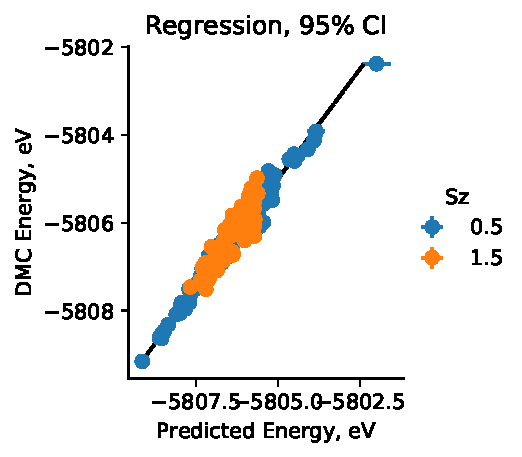
\includegraphics[width=\linewidth]{../qwalk/ub3lyp_s1_/analysis/regr_log.pdf}
  \caption{Prediction of linear regression on full set of samples.}
  \label{fig:Regression1}
\end{subfigure}%
\begin{subfigure}{.5\textwidth}
  \centering
  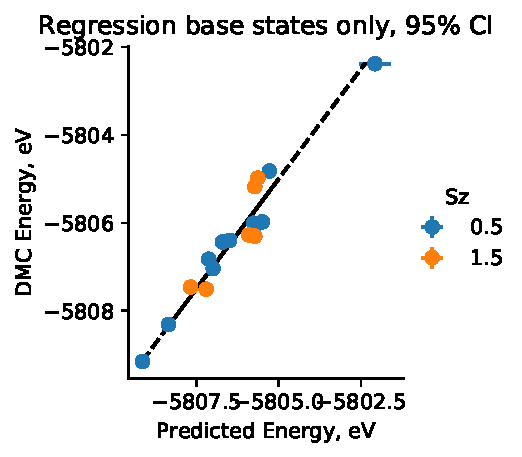
\includegraphics[width=\linewidth]{../qwalk/ub3lyp_s1_/analysis/regr_log_base.pdf}
  \caption{Prediction of linear regression on base states only.}
  \label{fig:Regression2}
\end{subfigure}
\label{fig:Regression}
\caption{Linear regression predictions for total energy compared to DMC energies.}
\end{figure}

%Figure 2
\begin{figure}[H]
\centering
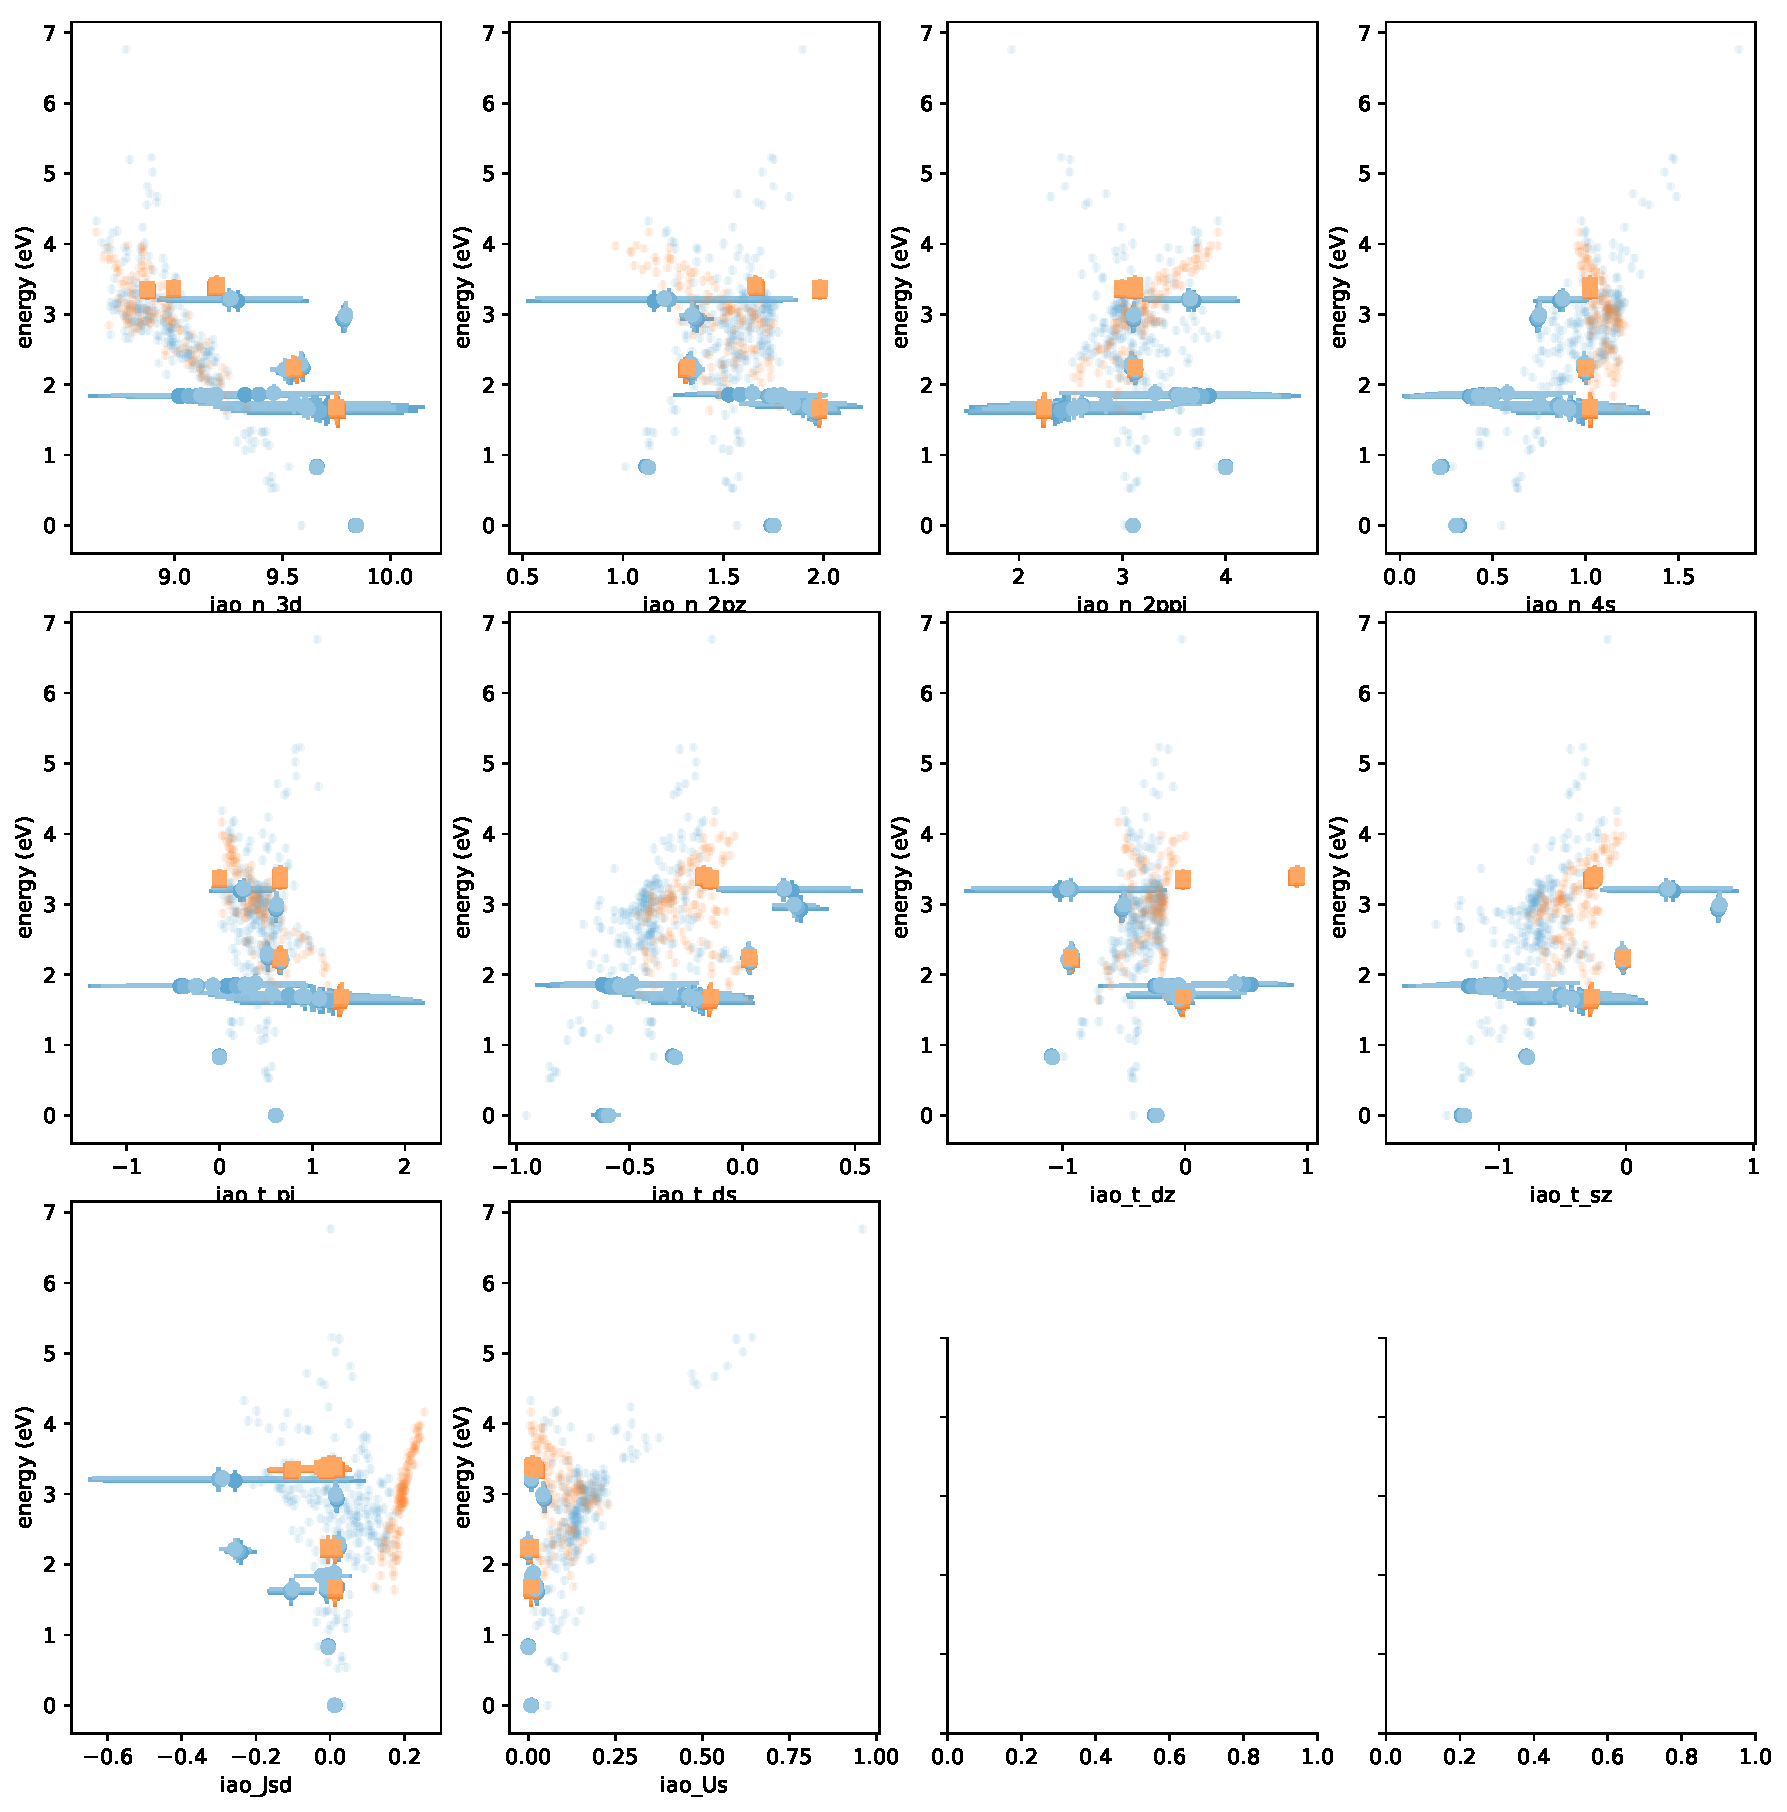
\includegraphics[width=\linewidth]{../qwalk/ub3lyp_s1_/analysis/ed_0_log.pdf}
\label{fig:ED}
\caption{Results for energies and 1-/2-body properties of eigenstates from exact diagonalization of our model Hamiltonian.}
\end{figure}

\section{Supplementary Material} 
%Supplementary Figure 1
\begin{figure}[H]
\centering
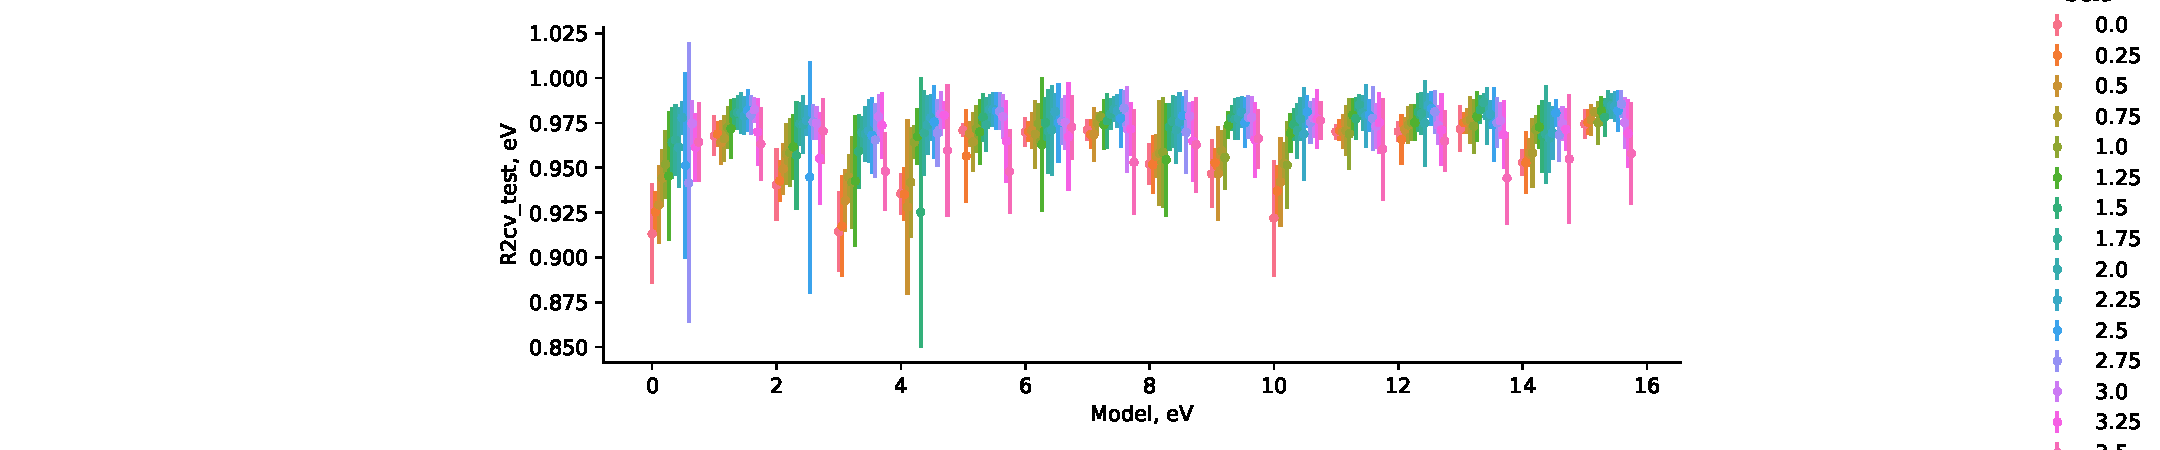
\includegraphics[width=\linewidth]{../qwalk/ub3lyp_s1_/analysis/r2_test.pdf}
\label{fig:OneParm}
\caption{Cross validated R2 scores for all sixteen models under consideration, hued by $\beta$.}
\end{figure}

%Supplementary Figure 2
\begin{figure}[H]
\centering
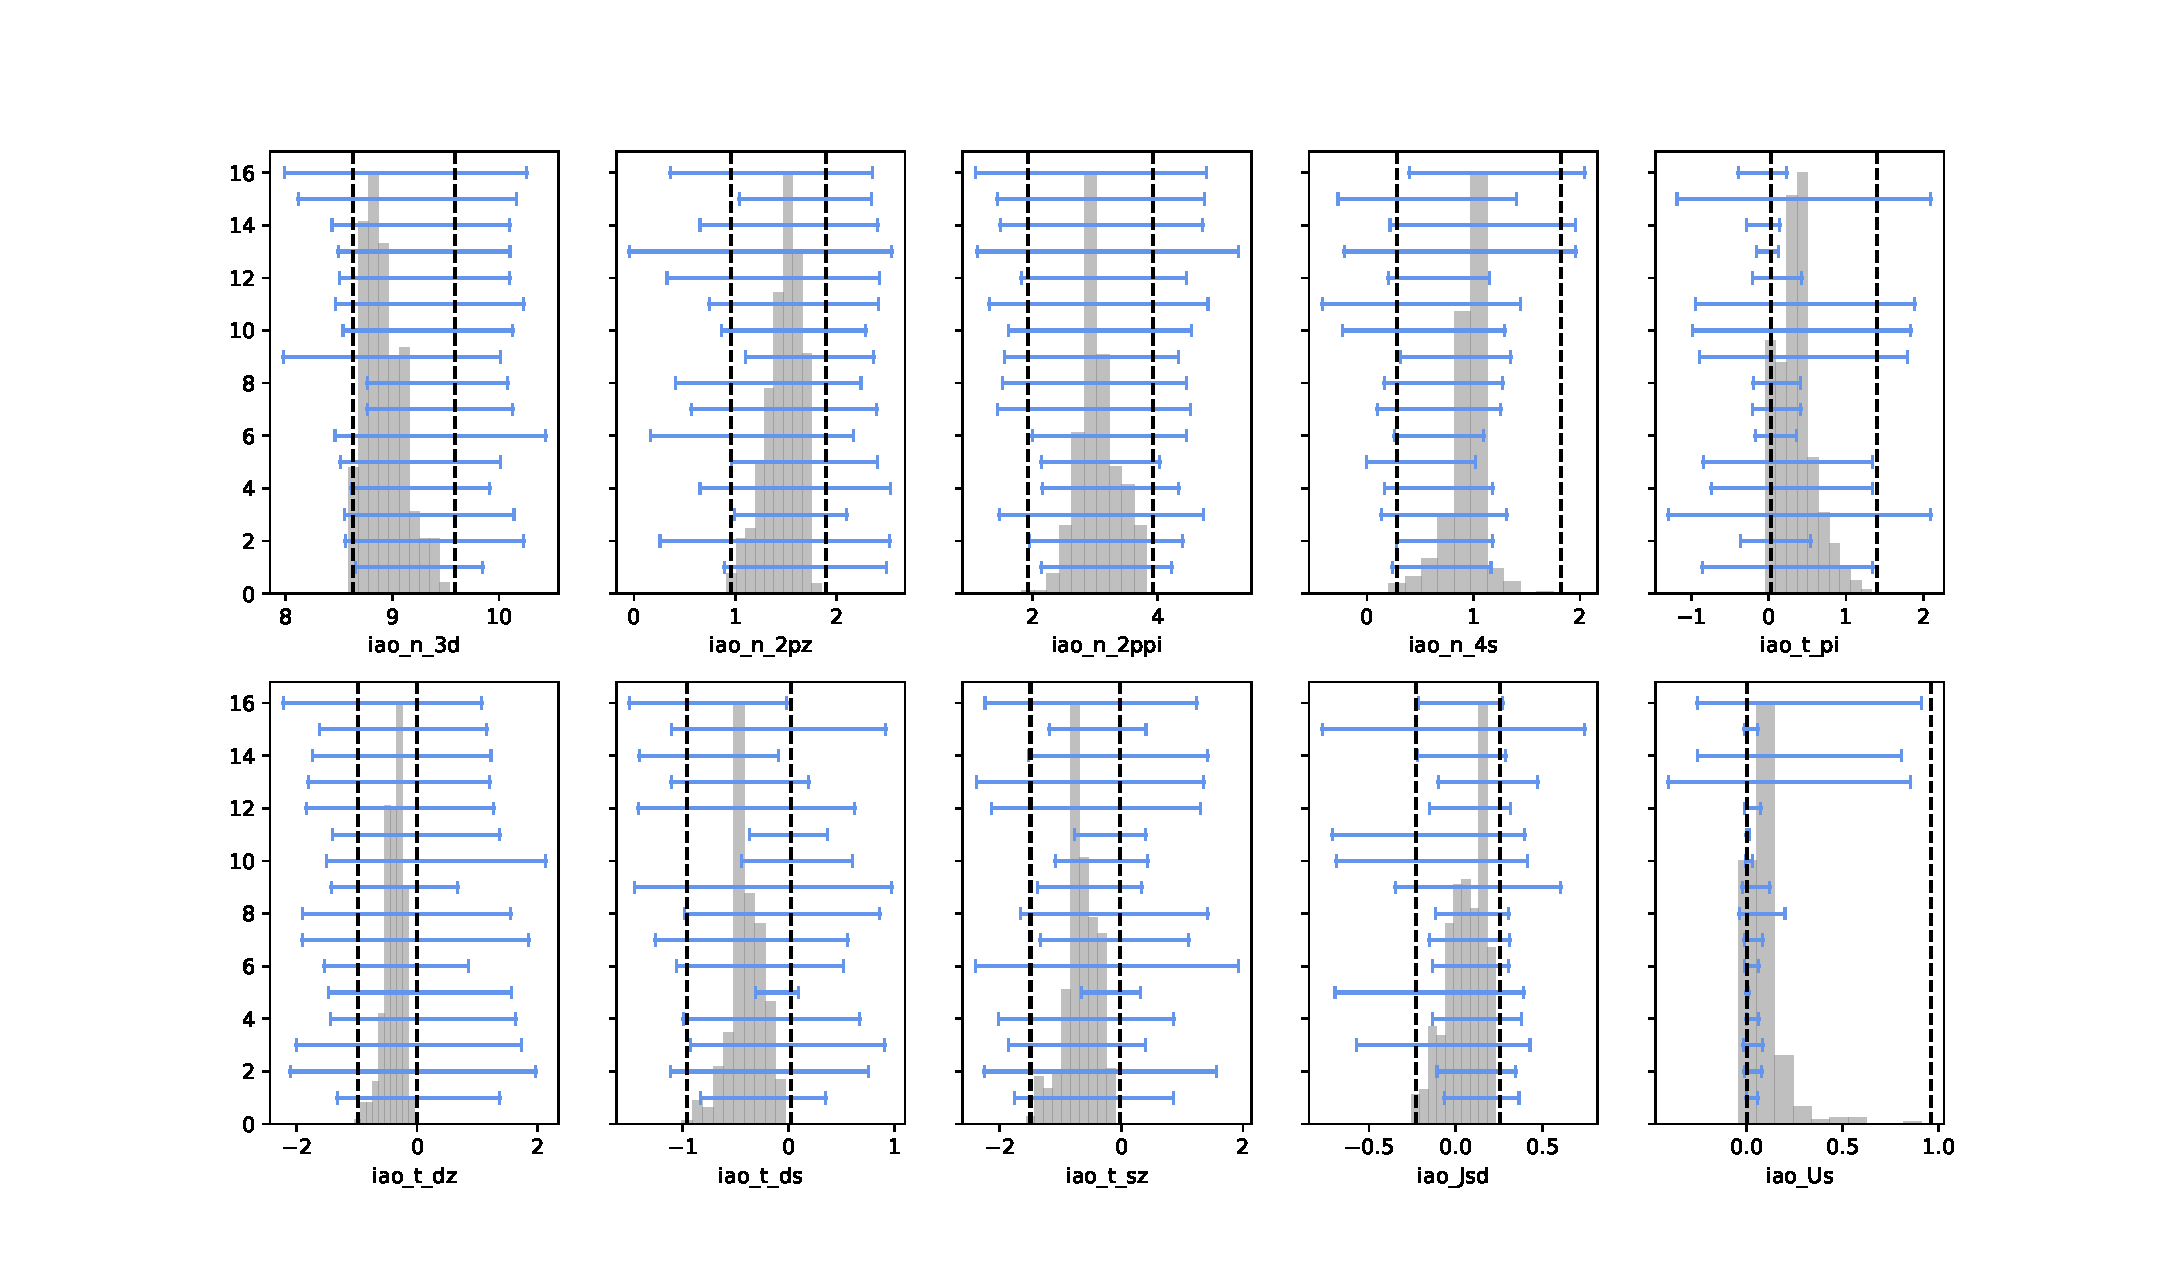
\includegraphics[width=\linewidth]{../qwalk/ub3lyp_s1_/analysis/Xerr.pdf}
\label{fig:Xerr}
\caption{Ranges of parameters from ED using the first 80 eigenstates compared against the ranges of the DMC training data.}
\end{figure}

%Supplementary Figure 3
\begin{figure}[H]
\centering
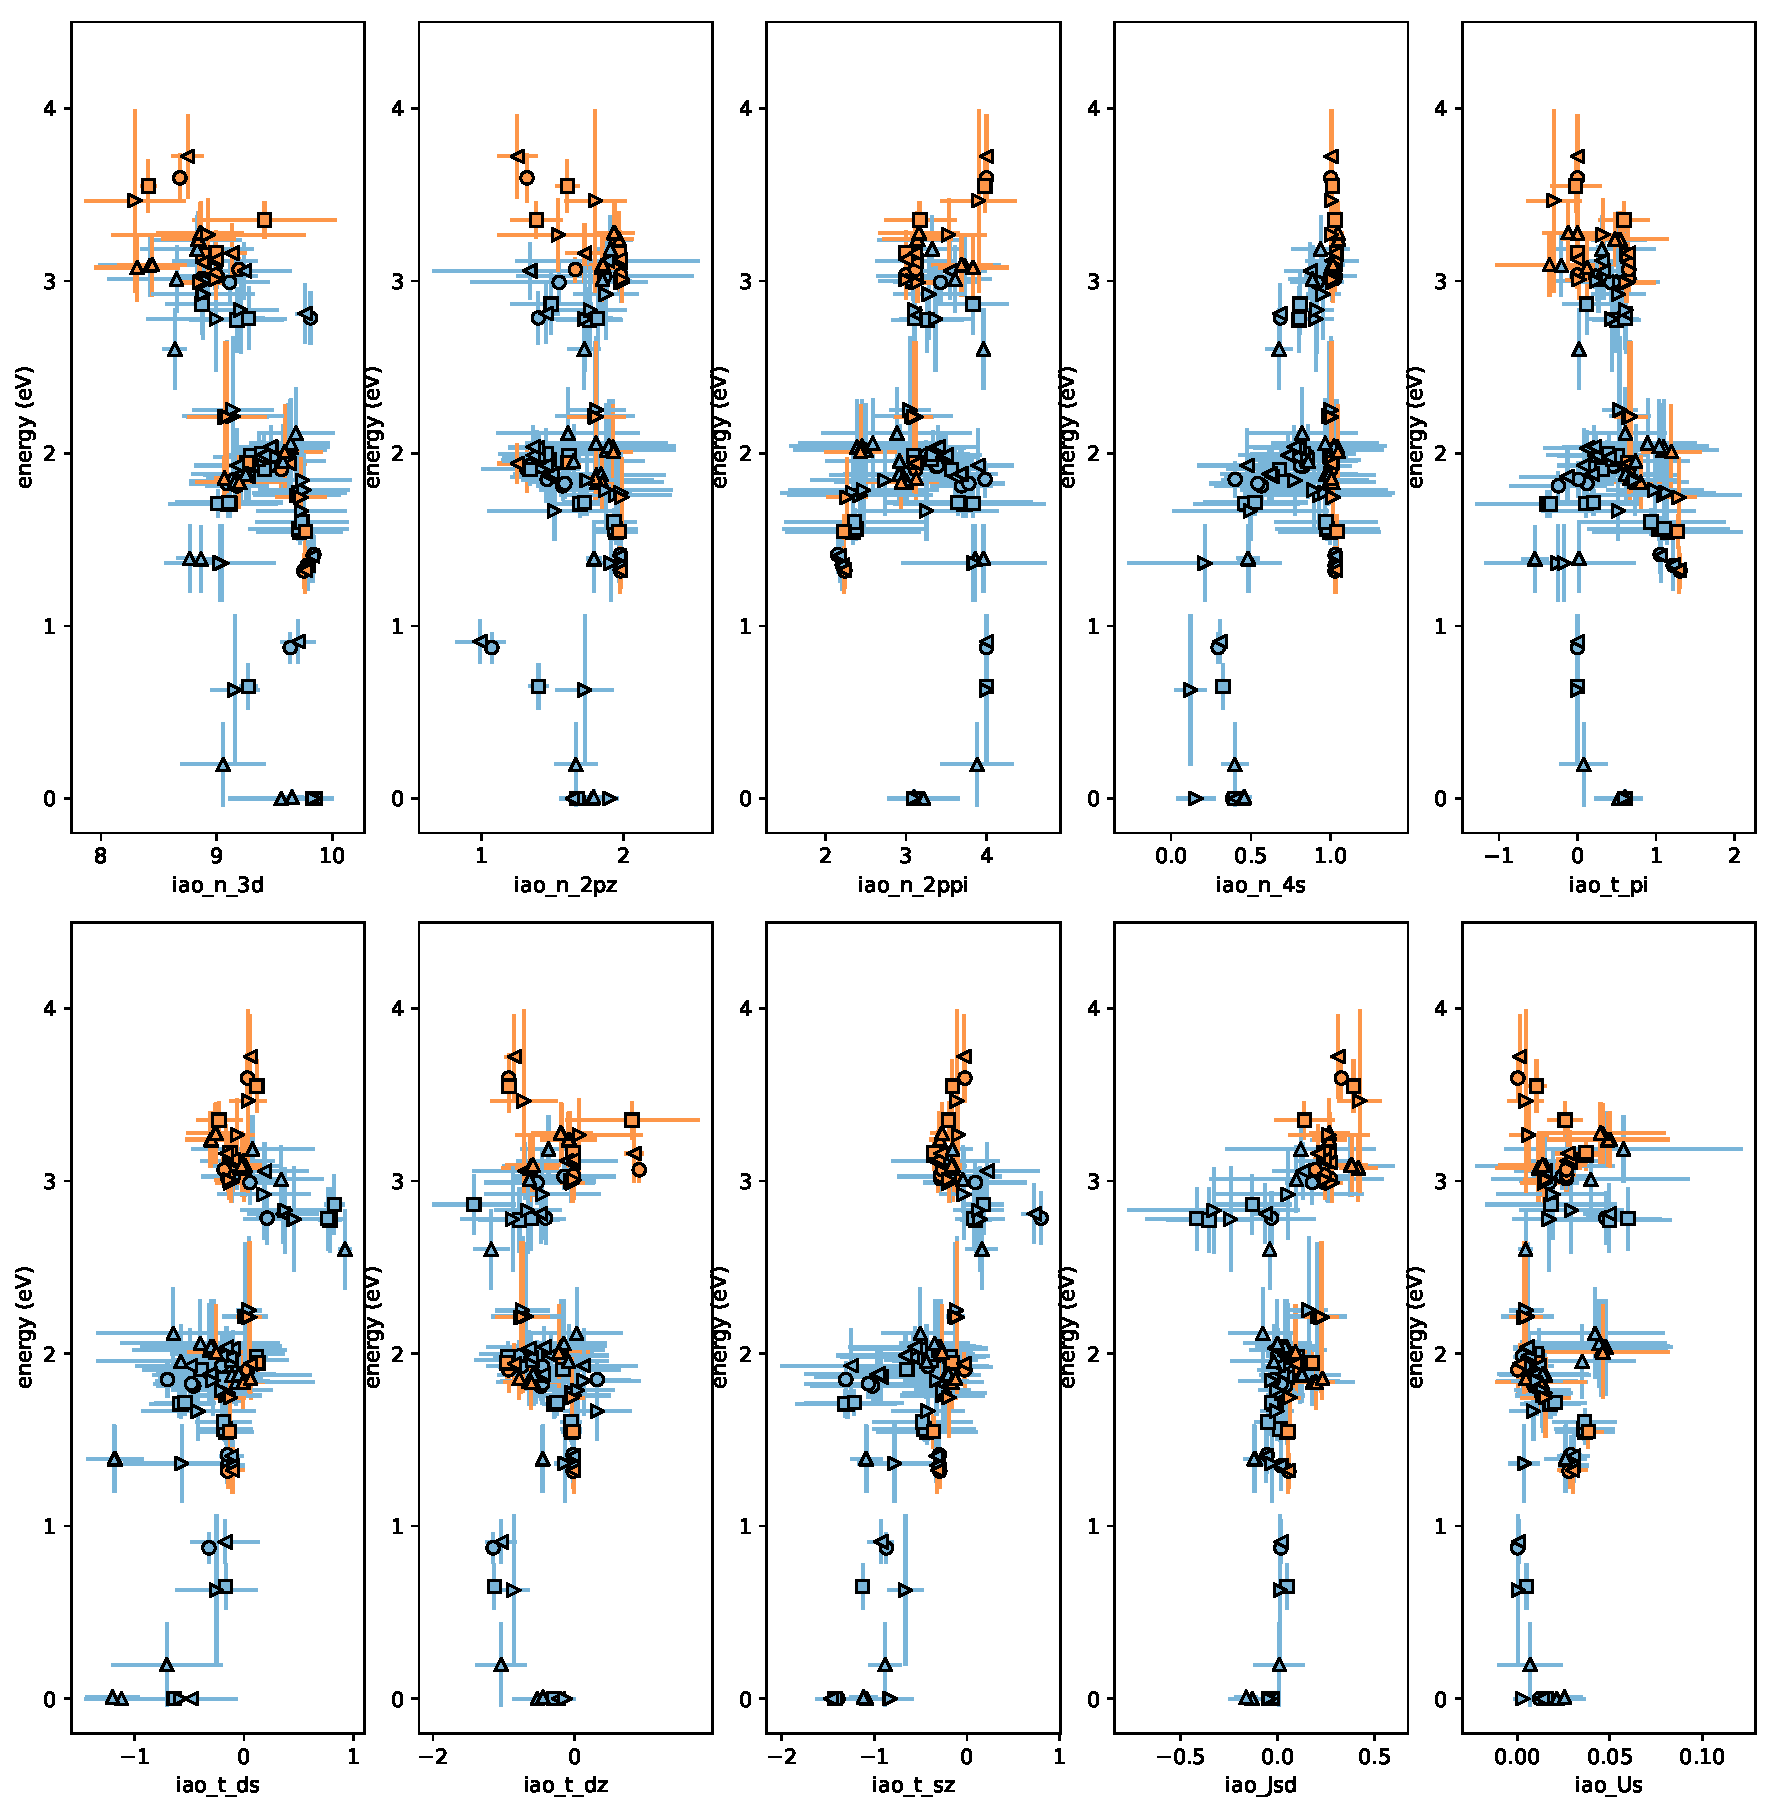
\includegraphics[width=0.9\linewidth]{../qwalk/ub3lyp_s1_/analysis/ed_combined_log.pdf}
\label{fig:ED_comp}
\caption{ED results for the four selected models, different models have different markers. Models with more parameter have larger error bars, but all three models have similar results within errorbars.}
\end{figure}


%Table 1
%\begin{figure}[H]
\begin{table}[H]
\centering
\begin{tabular}{l|lllll}
    & Model 0 & Model 2 & Model 3 & Model 8 & Model 14 \\ \hline
$\bar{\epsilon}_s$  & 3.0(1)  & 3.1(1)  & 3.0(1)  & 3.1(1)  & 2.9(1)   \\
$\bar{\epsilon}_\pi$ & 1.9(1)  & 1.7(1)  & 1.9(2)  & 1.4(2)  & 1.4(2)   \\
$\bar{\epsilon}_z$ & 0.8(1)  & 0.6(1)  & 0.8(2)  & 0.4(2)  & 0.6(2)   \\
$\bar{t}_{sz}$& 0       & -0.5(1) & 0       & -0.7(2) & -0.4(2)  \\
$\bar{t}_{sz}$& 0       & 0       & \textcolor{red}{-0.2(5)} & 0.8(4)  & \textcolor{red}{0.4(5)}   \\
$\bar{t}_{ds}$& 0       & 0       & 0       & 0       & 0.7(4)   \\
$\bar{t}_{\pi}$& 0       & 0       & 0       & 0       & 0        \\
$J_{sd}$ & -0.8(3) & -0.5(3) & -0.7(3) & -0.7(3) & -0.6(3)  \\
$U_s$  & 4.7(5)  & 4.2(6)  & 4.7(5)  & 4.0(5)  & 3.7(6)  
\end{tabular}
\label{fig:Table1}
\caption{Model parameters for models with appropriate descriptor ranges.}
\end{table}
%\end{figure} 
\end{document}